\documentclass{article}
\usepackage{amsmath,amsfonts,amsthm,amssymb}
\usepackage{fullpage,fancyheadings}
\usepackage[pdftex]{graphicx}
\usepackage[usenames,dvipsnames]{color}
\usepackage{listings}
\usepackage{courier}
\usepackage{ifthen}
\usepackage{setspace}
\usepackage{fancyhdr}
\usepackage{lastpage}
\usepackage{extramarks}
\usepackage{chngpage}
\usepackage{soul}
\usepackage{graphicx,float,wrapfig}

\topmargin=-0.45in      %
\evensidemargin=0in     %
\oddsidemargin=0in      %
\textwidth=6.5in        %
\textheight=9.0in       %
\headsep=0.25in         %

\pagestyle{fancyplain}
 
\fancyhf{}
 
\lhead{\fancyplain{}{Michael Carroll}}
\chead{\fancyplain{}{ELEC6410 - DSP}}
\rhead{\fancyplain{}{\today}}
\rfoot{\fancyplain{}{\thepage\ of \pageref{LastPage}}}

\sloppy
\definecolor{lightgray}{gray}{0.5}
\setlength{\parindent}{0pt}

\newcommand{\HRule}{\rule{\linewidth}{0.5mm}}
\definecolor{MyDarkGreen}{rgb}{0.0,0.4,0.0}

% For faster processing, load Matlab syntax for listings
\lstloadlanguages{Matlab}%
\lstset{language=Matlab,
        frame=single,
        basicstyle=\ttfamily,
        keywordstyle=[1]\color{Blue}\bf,
        keywordstyle=[2]\color{Purple},
        keywordstyle=[3]\color{Blue}\underbar,
        identifierstyle=,
        commentstyle=\usefont{T1}{pcr}{m}{sl}\color{MyDarkGreen}\small,
        stringstyle=\color{Purple},
        showstringspaces=false,
        tabsize=5,
        % Put standard MATLAB functions not included in the default
        % language here
        morekeywords={xlim,ylim,var,alpha,factorial,poissrnd,normpdf,normcdf},
        % Put MATLAB function parameters here
        morekeywords=[2]{on, off, interp},
        % Put user defined functions here
        morekeywords=[3]{FindESS},
        morecomment=[l][\color{Blue}]{...},
        numbers=left,
        firstnumber=1,
        numberstyle=\tiny\color{Blue},
        stepnumber=5
        }



\begin{document}
  
\section*{ELEC6410 Project 2}

\subsection*{Question 1}

\begin{par}
Let $y[n] - 0.9y[n-1] + 0.7y[n-2] = x[n] + 0.5x[n-1] + 0.3x[n-2]$. This difference equation can be implemented using the filter command.  Find the vectors a and b that represent that difference equation above for the filter command.
\end{par} \vspace{1em}


\subsection*{Solution}

\begin{par}
Using the properties of the Fourier transform, the difference equation can be rearranged to the following:
\end{par} \vspace{1em}
\begin{par}
$$\frac{Y(e^{j\omega})}{X(e^{j\omega})} =
\frac{1 + 0.5e^{-j\omega} + 0.3e^{-2j\omega}}
{1 - 0.9e^{-j\omega} + 0.7e^{-2j\omega}}$$
\end{par} \vspace{1em}
\begin{par}
Yielding the following two vectors, with vector "a" representing the y coefficients, and vector "b" representing the x coefficiencts:
\end{par} \vspace{1em}
\begin{lstlisting}[language=matlab]
a = [1 -0.9, 0.7];
b = [1, 0.5, 0.3];
\end{lstlisting}

\subsection*{Question 2}

\begin{par}
Calculate $h[n]$ analytically for the difference equation above.  Your answer should be a functional expression.  Hint: You may find the residuez function useful.  Note that the initial expression may come out with complex components.  However, it is possible to simplify it into an expression that is real.
\end{par} \vspace{1em}


\subsection*{Solution}

\begin{par}
Using the derived equation in the Fourier domain from Question 1, the impulse response of h[n] may be calculated.
\end{par} \vspace{1em}
\begin{par}
$$H(e^{j\omega}) = \frac{Y(e^{j\omega})}{X(e^{j\omega})} =
\frac{1 + 0.5e^{-j\omega} + 0.3e^{-2j\omega}}
{1 - 0.9e^{-j\omega} + 0.7e^{-2j\omega}}$$
\end{par} \vspace{1em}
\begin{par}
Using partial fraction expansion and the residuez command in MATLAB, this yields the equation:
\end{par} \vspace{1em}
\begin{par}
$$H(e^{j\omega}) = \frac{R(1)}{1-P(1)e^{-jw}} + \frac{R(2)}{1-P(2)e^{-j\omega}} +
k$$
\end{par} \vspace{1em}
\begin{par}
Which equals:
\end{par} \vspace{1em}
\begin{par}
$$H(e^{j\omega}) = \frac{0.2857 - 0.8101j}{1- (0.45 + 0.7053j)e^{-j\omega}} +
\frac{0.2857 + 0.8101j}{1 - (0.45 - 0.7053j)e^{-j\omega}} + 0.4286$$
\end{par} \vspace{1em}
\begin{par}
Using the Inverse DTFT yields:
\end{par} \vspace{1em}
\begin{par}
$$h[n] = 0.4286\delta[n] + (0.2857 - 0.8101j)(0.45 + 0.7053j)^{n}\mu[n] +
(0.2857 + 0.8101j)(0.45 - 0.7053j)^{n}\mu[n]$$
\end{par} \vspace{1em}
\begin{par}
Using the exponential representation of complex numbers:
\end{par} \vspace{1em}
\begin{par}
$$h[n] = 0.4286\delta[n] + (0.859e^{-1.2317j})(0.8366e^{j})^{n}\mu[n] +
(0.859e^{1.2317j})(0.8366e^{-j})^{n}\mu[n]$$
\end{par} \vspace{1em}
\begin{par}
Combining some of the exponential terms:
\end{par} \vspace{1em}
\begin{par}
$$h[n] = 0.4286\delta[n] + 0.718e^{(-1.2317 + n)j} + 0.718e^{(1.2317 -
n)j}\mu[n]$$
\end{par} \vspace{1em}
\begin{par}
Using Euler's Identity:
\end{par} \vspace{1em}
\begin{par}
$$h[n] = 0.4286\delta[n] + 1.436\cos{(n - 1.2317)}\mu[n]$$
\end{par} \vspace{1em}
\begin{lstlisting}[language=matlab]
[r,p,k] = residuez(b,a)
\end{lstlisting}

        \color{lightgray} \begin{verbatim}
r =

   0.2857 - 0.8101i
   0.2857 + 0.8101i


p =

   0.4500 + 0.7053i
   0.4500 - 0.7053i


k =

    0.4286

\end{verbatim} \color{black}
    
\subsection*{Question 3}

\begin{par}
Create an impulse (not a pulse!) of length 100.  Recall that systems described by linear constant-coefficient difference equations are LSI systems (assuming initial rest conditions).  Characterize the LSI system above by finding the first 100 points of the impulse response using filter, and plot the result with stem.
\end{par} \vspace{1em}


\subsection*{Solution}

\begin{par}
The system was characterized using the filter function to generate an impulse response for the system.  The impulse response is plotted in Figure ~\ref{fig:impresp}.
\end{par} \vspace{1em}
\begin{lstlisting}[language=matlab]
figure(1);
impulse = [1, zeros(1,99)];

impulseResponse = filter(b,a,impulse);

stem(impulseResponse);
title('Impulse Response of y[n]');
xlabel('Samples');ylabel('Amplitude');
\end{lstlisting}

\begin{figure}[here]
	\begin{center}
		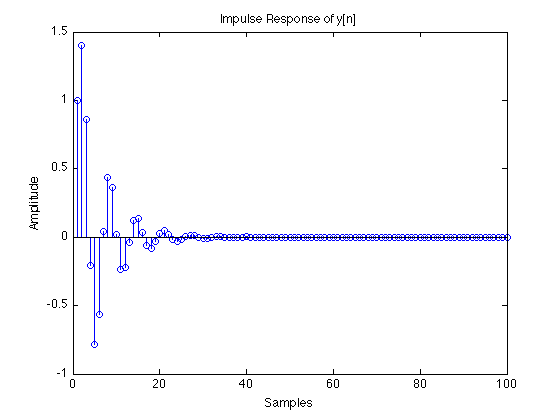
\includegraphics [width=5in]{Project2_01.png}
		\caption{Impulse response of y[n]}
		\label{fig:impresp}
	\end{center}
\end{figure}

\subsection*{Question 4}

\begin{par}
Examine two ways of implementing an LSI system:
\end{par}
\begin{enumerate}
\setlength{\itemsep}{-1ex}
   \item Create a pulse of width 10 and zeropadded to a total length of 100.
   \item Find the response of the system to this input pulse using conv by convolving with the impulse response.
   \item Find the response of the system to this input pulse using filter by filtering with the difference equation.
   \item Explain any differences you observe between these two results.
\end{enumerate}


\subsection*{Solution}

\begin{par}
The system's response to a pulse of width 10 was generated using the impulse reponse of the system, characterized in the previous question.
\end{par} \vspace{1em}
\begin{par}
The filter command was then used to generate a similar response to the pulse of width 10.
\end{par} \vspace{1em}
\begin{par}
Both responses are included in Figure ~\ref{fig:impcomp}.  The convolution response ends up containing a higher number of samples due to the nature of the operating.  Convolving the two samples together, each of length 100, will yield a sample with length 199.  The 100 points that the filter response generated are identical to the first 100 points of the convolution function, just truncated at the 101st sample.
\end{par} \vspace{1em}
\begin{lstlisting}[language=matlab]
pulse = [ones(1,10),zeros(1,90)];
convolutionResults = conv(pulse,impulseResponse);
filterResults = filter(b,a,pulse);

figure(2);
subplot(2,1,1);
stem(convolutionResults);
title('LSI System Response using MATLAB conv() function');
xlabel('Samples');ylabel('Amplitude');
subplot(2,1,2);
stem(filterResults);
title('LSI System Response using MATLAB filter() function');
xlabel('Samples');ylabel('Amplitude');
\end{lstlisting}

\begin{figure}[here]
	\begin{center}
		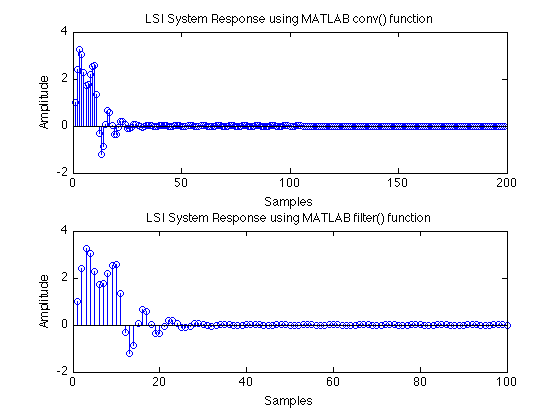
\includegraphics [width=5in]{Project2_02.png}
		\caption{Comparison of conv() and filter() impulse responses}
		\label{fig:impcomp}
	\end{center}
\end{figure}

\newpage
\subsection*{Question 5}

\begin{par}
Examine the frequency response:
\end{par} \vspace{1em}
\begin{enumerate}
\setlength{\itemsep}{-1ex}
   \item Find an expression for the frequency response of the system described by the difference equation given.
   \item Use the command freqz to plot the magnitude and phase response of the system.
   \item Is this system more of a highpass, a lowpass, or a bandpass filter? Explain your answer.
\end{enumerate}


\subsection*{Solution}

\begin{par}
The frequency response of the system was found as part of the derivation of h[n].
\end{par} \vspace{1em}
\begin{par}
$$H(e^{j\omega}) = \frac{Y(e^{j\omega})}{X(e^{j\omega})} =
\frac{1 + 0.5e^{-j\omega} + 0.3e^{-2j\omega}}
{1 - 0.9e^{-j\omega} + 0.7e^{-2j\omega}}$$
\end{par} \vspace{1em}
\begin{par}
From looking at the graph of the magnitude and phase response in Figure ~\ref{fig:freqz}, then system appears to be a low-pass filter, but it is important to remember that the frequency response is periodic in $\omega$ with a period of $2\pi$.  This makes the filter a bandpass filter.
\end{par} \vspace{1em}
\begin{lstlisting}[language=matlab]
figure(3);
freqz(b,a);
title('Magnitude and Phase Response');
\end{lstlisting}

\begin{figure}[here]
	\begin{center}
		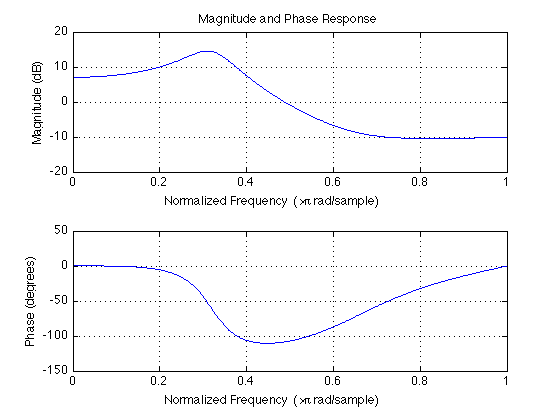
\includegraphics [width=5in]{Project2_03.png}
		\caption{Magnitude and phase response of the filter using the freqz() command}
		\label{fig:freqz}
	\end{center}
\end{figure}

\newpage
\subsection*{Question 6}

\begin{par}
Examine the reponse to two sine waves:
\end{par} \vspace{1em}
\begin{enumerate}
\setlength{\itemsep}{-1ex}
   \item Create two signals $x_{1}[n] = \cos(0.32\pi n)$ and $x_{2}[n] = \cos(0.8 \pi n)$, both of length 100.
   \item Filter each signal separately with the filter defined in Step 1, and plot them.
   \item Explain the outputs you observe in terms of the frequency magnitude response of the system.
   \item Now add the two signals together and filter the sum of the two. Explain the output in light of your previous observations.
\end{enumerate}


\subsection*{Solution}

\begin{par}
To determine the effect of the filter on the two signals, it is important to note where in the magnitude response that the two signals fall.  The first signal, x1, falls at $0.32\pi$ radians, which is in the middle of the pass band of the filter (about 15dB gain).  The second signal, x2, falls at $0.8\pi$ radians, which is in the middle of the stop band of the filter (about -10dB attenuation).
\end{par} \vspace{1em}
\begin{par}
Using this knowledge, the output of the filter for the two different input signals can be seen in Figure ~\ref{fig:indresp}.  As expected, the first signal, x1, has a significant gain in amplitude, reaching a value of almost 5. The second signal, x2, has a decrease in amplitude, barely reaching 0.5.
\end{par} \vspace{1em}
\begin{par}
The combination of the two signals in Figure ~\ref{fig:combresp} yields the same results, with the major peaks in the signal coming mainly from the contributions of signal x1.
\end{par} \vspace{1em}
\begin{lstlisting}[language=matlab]
x1 = cos(0.32*pi*(0:1:100));
x2 = cos(0.80*pi*(0:1:100));

figure(4);
subplot(2,1,1);
stem(filter(b,a,x1));
title('Filter Response to x1');xlabel('Samples');ylabel('Amplitude');
subplot(2,1,2);
stem(filter(b,a,x2));
title('Filter Response to x2');xlabel('Samples');ylabel('Amplitude');

figure(5);
stem(filter(b,a,x1+x2));
title('Filter Reponse to Combined x1 and x2');
xlabel('Samples');ylabel('Amplitude');
\end{lstlisting}

\begin{figure}[here]
	\begin{center}
		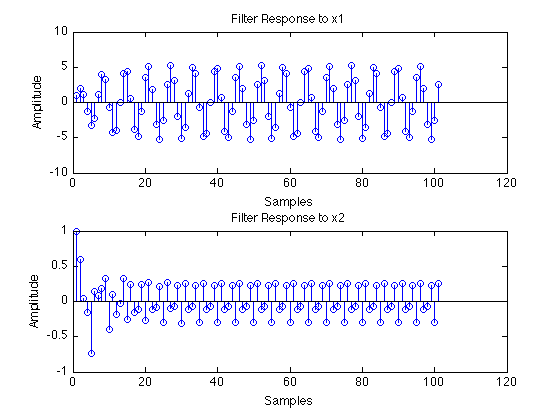
\includegraphics [width=5in]{Project2_04.png}
		\caption{Filter response to individual input signals x1 and x2}
		\label{fig:indresp}
	\end{center}
\end{figure}

\begin{figure}[here]
	\begin{center}
		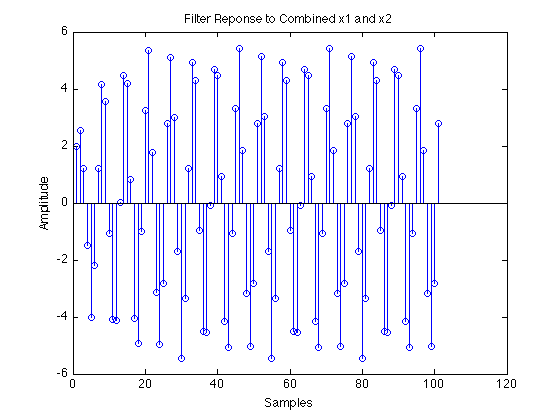
\includegraphics [width=5in]{Project2_05.png}
		\caption{Filter response to combined input signals x1 and x2}
		\label{fig:combresp}
	\end{center}
\end{figure}

\end{document}
    
